\section{Question 2} 
\label{sec:Q2}

%-------------------------------------------------------------------------
\subsection{Training Time}

\begin{figure}[h]
	\centering
	%\fbox{\rule{0pt}{2in} \rule{0.9\linewidth}{0pt}}
	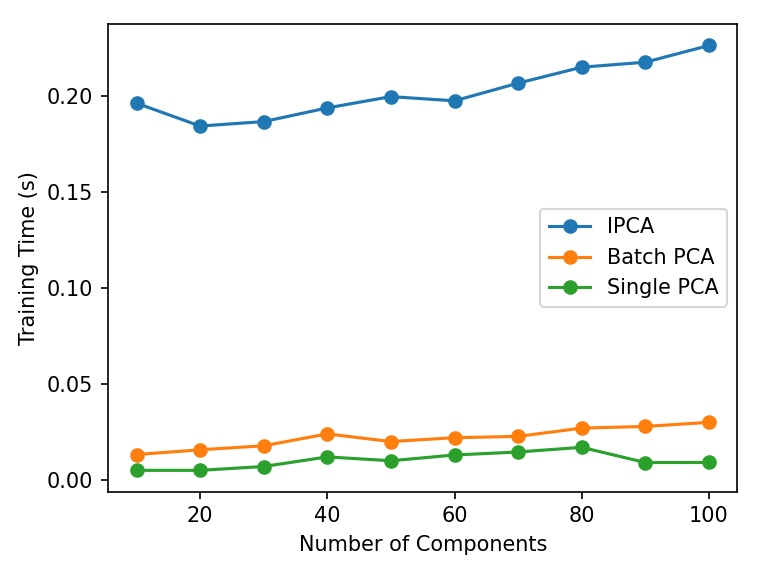
\includegraphics[width=0.8\linewidth]{Ressources/Q2_time.png}
	
	\caption{Q2\_time}
	\label{fig:Q2_time}
\end{figure}

Figure~\ref{fig:Q2_time} shows the change in training time for the three methods as the number of principal components increases. It can be seen that IPCA (blue line) is higher in training time relative to Batch PCA and Single PCA, mainly because IPCA processes data in multiple steps/batches and each batch requires updating the components. Both Batch PCA and Single PCA have shorter training times, with Single PCA having the lowest training time. Because single PCA only uses the first subset, which has the least computation.

%-------------------------------------------------------------------------
\subsection{Reconstruction Error}

\begin{figure}[h]
	\centering
	%\fbox{\rule{0pt}{2in} \rule{0.9\linewidth}{0pt}}
	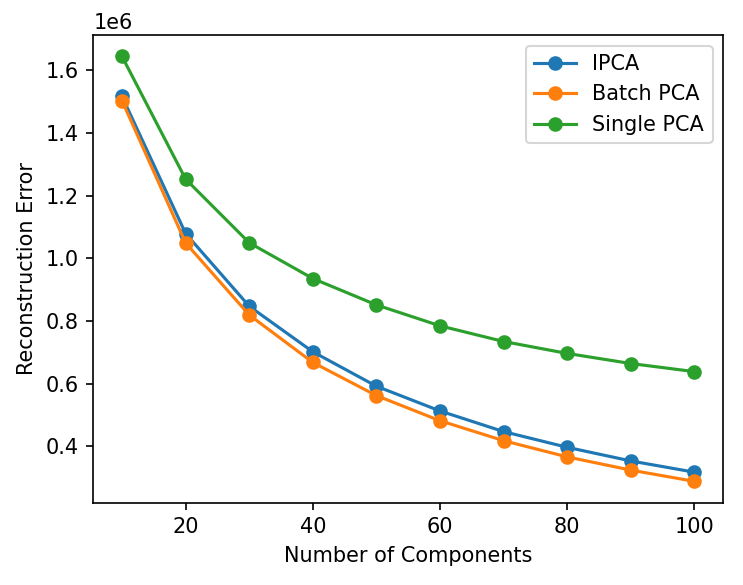
\includegraphics[width=0.8\linewidth]{Ressources/Q2_error.png}
	
	\caption{Q2\_error}
	\label{fig:Q2_error}
\end{figure}
Figure~\ref{fig:Q2_error} shows the reconstruction errors of the three methods with different numbers of principal components. As the number of principal components increases, the reconstruction errors of all three methods decrease, which indicates that the higher the number of principal components, the higher the accuracy of the model in reconstructing the data.The reconstruction errors of IPCA and Batch PCA perform similarly and are better than those of Single PCA, and the difference is more obvious especially when the number of principal components is small.

%-------------------------------------------------------------------------
\subsection{Accuracy}

\begin{figure}[H]
	\centering
	%\fbox{\rule{0pt}{2in} \rule{0.9\linewidth}{0pt}}
	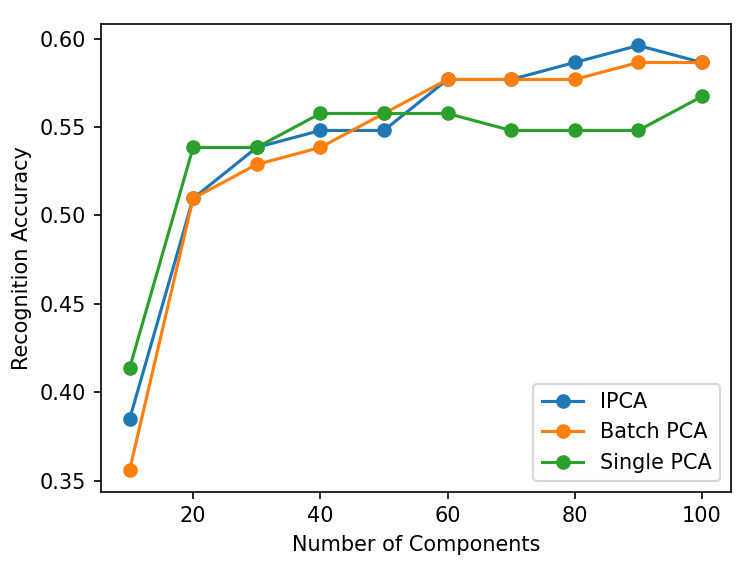
\includegraphics[width=0.8\linewidth]{Ressources/Q2_accuracy.png}
	
	\caption{Q2\_accuracy}
	\label{fig:Q2_accuracy}
\end{figure}
Figure~\ref{fig:Q2_accuracy} shows the recognition accuracies of the three methods. As the number of principal components increases, the recognition accuracies of the three methods generally increase, indicating that more principal components help to improve the classification accuracy. IPCA and Batch PCA perform close to each other and slightly better than Single PCA, especially when the number of principal components is higher.


%-------------------------------------------------------------------------
\subsection{Discussions}

IPCA and Batch PCA perform close to each other in terms of reconstruction error and recognition accuracy, but the training time for IPCA is slightly higher. Single PCA is lower in reconstruction error and recognition accuracy, indicating that it is slightly less effective in retaining key feature information, but has the lowest training time.

But most importantly IPCA is more suitable for large scale datasets and online learning. It does not need all observations at once - thus, reducing storage requirements and making large problems feasible.

And obviously, the number of principal components retained by PCA is one of the important parameters affecting accuracy. But as it increases, it has less effect on accuracy. The first few components often contain most of the information needed for accurate predictions. Adding more components contributes less new, valuable information, leading to less accuracy improvement.
\newline